% $Header: /cvsroot/latex-beamer/latex-beamer/solutions/generic-talks/generic-ornate-15min-45min.en.tex,v 1.5 2007/01/28 20:48:23 tantau Exp $

\include{graphics}
\documentclass{beamer}

% This file is a solution template for:

% - Giving a talk on some subject.
% - The talk is between 15min and 45min long.
% - Style is ornate.



% Copyright 2004 by Till Tantau <tantau@users.sourceforge.net>.
%
% In principle, this file can be redistributed and/or modified under
% the terms of the GNU Public License, version 2.
%
% However, this file is supposed to be a template to be modified
% for your own needs. For this reason, if you use this file as a
% template and not specifically distribute it as part of a another
% package/program, I grant the extra permission to freely copy and
% modify this file as you see fit and even to delete this copyright
% notice. 


\mode<presentation>
{
  \usetheme{Warsaw}
  % or ...

  \setbeamercovered{transparent}
  % or whatever (possibly just delete it)
}


\usepackage[english]{babel}
% or whatever

\usepackage[latin1]{inputenc}
% or whatever

%Joe
%\usepackage{times}
%\usepackage[T1]{fontenc}
% Or whatever. Note that the encoding and the font should match. If T1
% does not look nice, try deleting the line with the fontenc.


\title[] % (optional, use only with long paper titles)
{Shortest-Path}

\subtitle
{Weighted Graphs, Djikstra's Algorithm, and Traveling Salesmen} % (optional)

\author{Joe Smith} % (optional, use only with lots of authors)
% - Use the \inst{?} command only if the authors have different
%   affiliation.

\institute[] % (optional, but mostly needed)
{
  Department of Computer Science\\
  Chapman University}
% - Use the \inst command only if there are several affiliations.
% - Keep it simple, no one is interested in your street address.

\date[] % (optional)
{Discrete Mathematics\\ \today}

%\subject{Talks}
% This is only inserted into the PDF information catalog. Can be left
% out. 



% If you have a file called "university-logo-filename.xxx", where xxx
% is a graphic format that can be processed by latex or pdflatex,
% resp., then you can add a logo as follows:

 \pgfdeclareimage[height=0.5cm]{university-logo}{chapman}
 \logo{\pgfuseimage{university-logo}}



% Delete this, if you do not want the table of contents to pop up at
% the beginning of each subsection:
\AtBeginSubsection[]
{
  \begin{frame}<beamer>{Outline}
    \tableofcontents[currentsection,currentsubsection]
  \end{frame}
}


% If you wish to uncover everything in a step-wise fashion, uncomment
% the following command: 

%\beamerdefaultoverlayspecification{<+->}


\begin{document}

\begin{frame}
  \titlepage
\end{frame}

\begin{frame}{Outline}
  \tableofcontents
  % You might wish to add the option [pausesections]
\end{frame}


% Since this a solution template for a generic talk, very little can
% be said about how it should be structured. However, the talk length
% of between 15min and 45min and the theme suggest that you stick to
% the following rules:  

% - Exactly two or three sections (other than the summary).
% - At *most* three subsections per section.
% - Talk about 30s to 2min per frame. So there should be between about
%   15 and 30 frames, all told.

\section{Weighted Graphs}

%\subsection[Short First Subsection Name]{First Subsection Name}
\subsection{Background}

\begin{frame}{Heavy Lifting}
  % - A title should summarize the slide in an understandable fashion
  %   for anyone how does not follow everything on the slide itself.

  \begin{itemize}
  \item
    A \alert{Weighted Graph} is a graph that has a number assigned to each edge.
  \item
    This number can mean cost, distance, or response time.
  \end{itemize}
\end{frame}

\begin{frame}{Different Lengths}

  \begin{itemize}
  \item
	The \alert{length} of a path in a weighted graph is the sum of the weights of the edges of this path.
  \item 
	In a typical graph, the \alert{length} of a path refers to the number of edges.
  \end{itemize}
\end{frame}


\begin{frame}{Example}
	\centerline{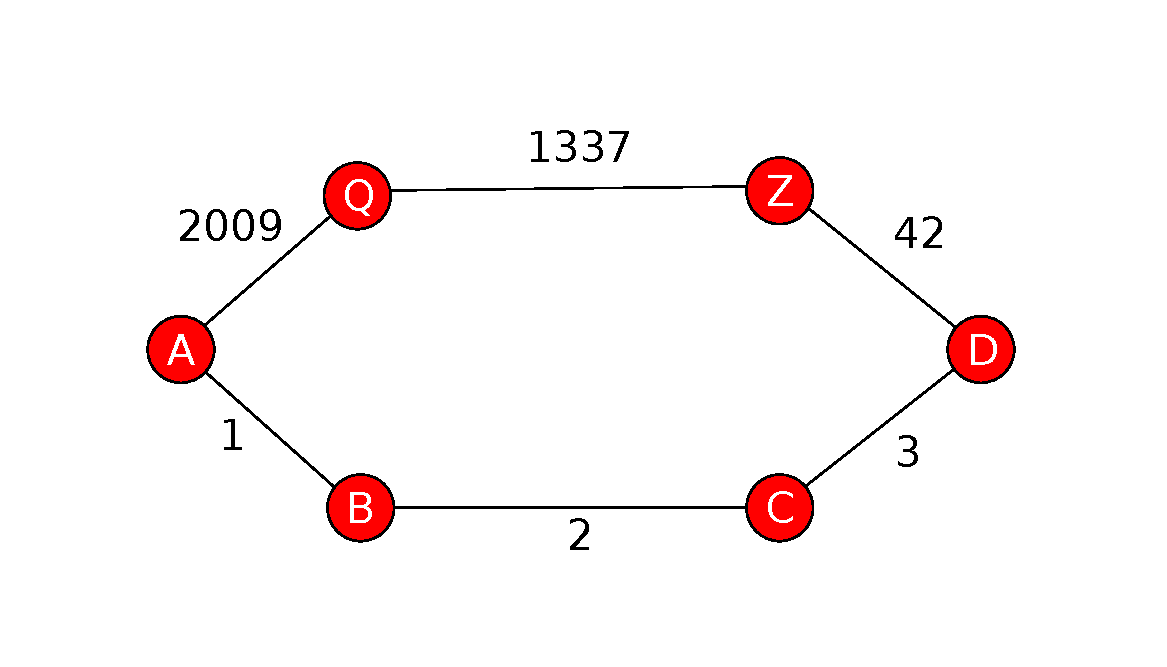
\includegraphics[width=3.5in]{weighted_ex_1.pdf}}
	\begin{itemize}
	\item
		What is the shortest path from A to D?
	\item
		ABCD
	\end{itemize}
\end{frame}

\subsection{Clicker Questions}
\begin{frame}{Shortest Path Between...}
	\centerline{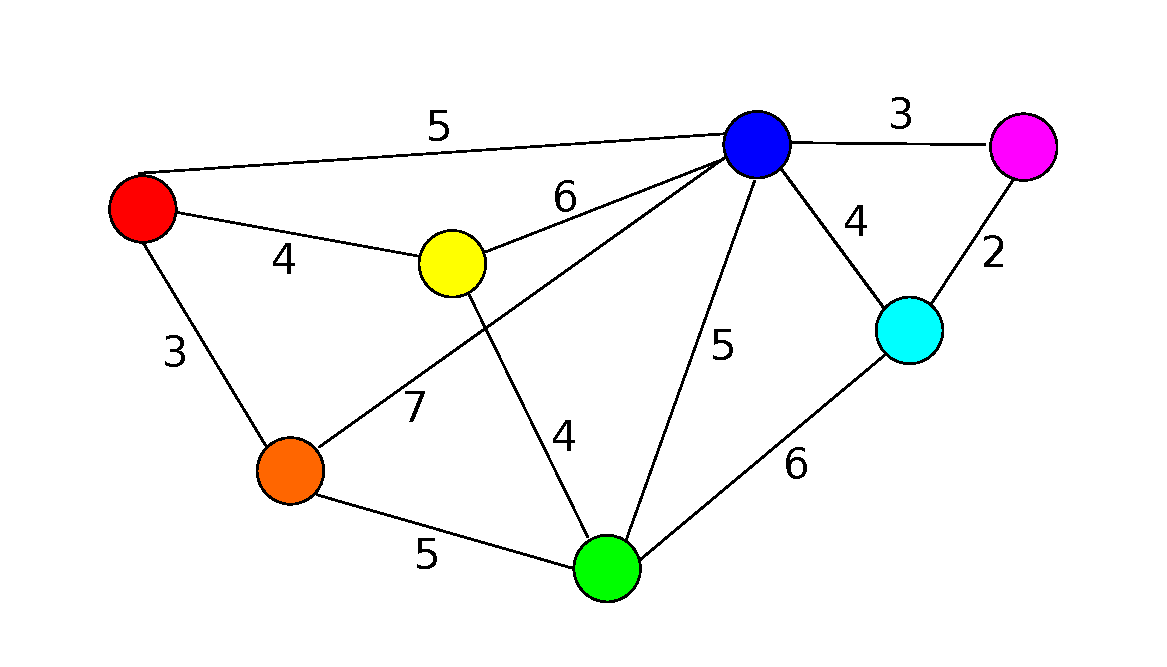
\includegraphics[width=3.0in]{weighted.pdf}}
	\textit{Red and Purple?}
        \begin{itemize}
	\item
		1. Red-Blue-Purple
	\item
		2. Red-Yellow-Blue-Indigo-Purple
	\item
		3. Red-Orange-Green-Indigo-Purple
	\item
		4. Red-Yellow-Green-Blue-Purple
	\end{itemize}
\end{frame}

\begin{frame}{Shortest Path Between...}
	\centerline{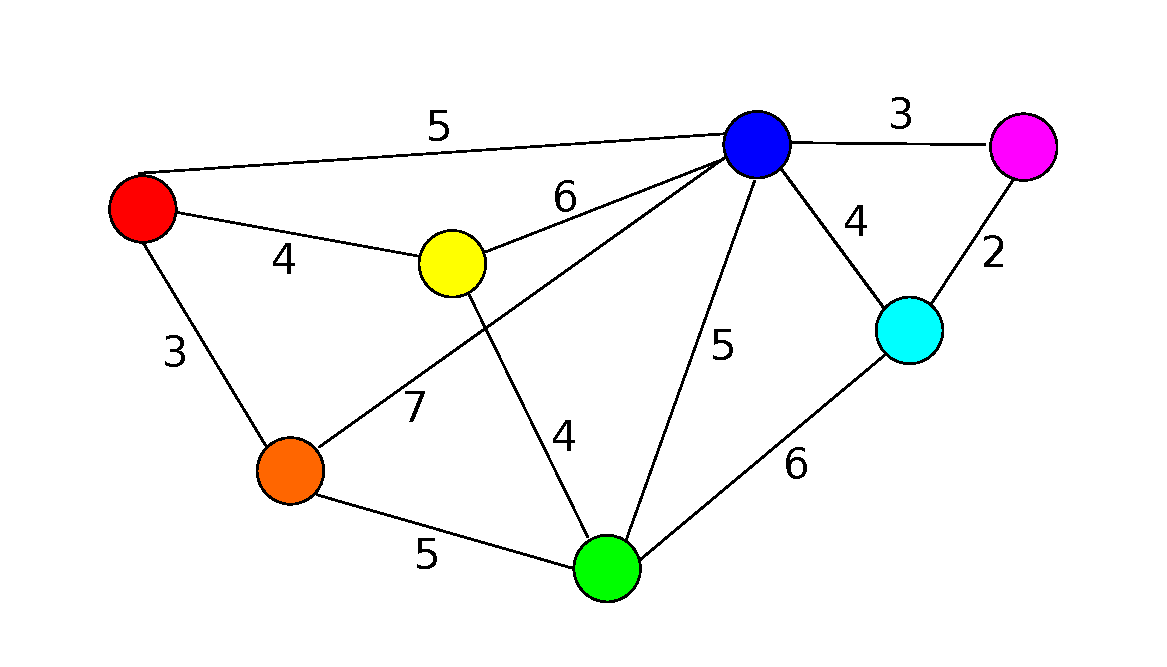
\includegraphics[width=3.0in]{weighted.pdf}}
	\textit{Red and Purple?}
        \begin{itemize}
	\item
		\alert{1. Red-Blue-Purple}
	\item
		2. Red-Yellow-Blue-Indigo-Purple
	\item
		3. Red-Orange-Green-Indigo-Purple
	\item
		4. Red-Yellow-Green-Blue-Purple
	\end{itemize}
\end{frame}

%%%NEW QUESTION
\begin{frame}{Shortest Path Between...}
	\centerline{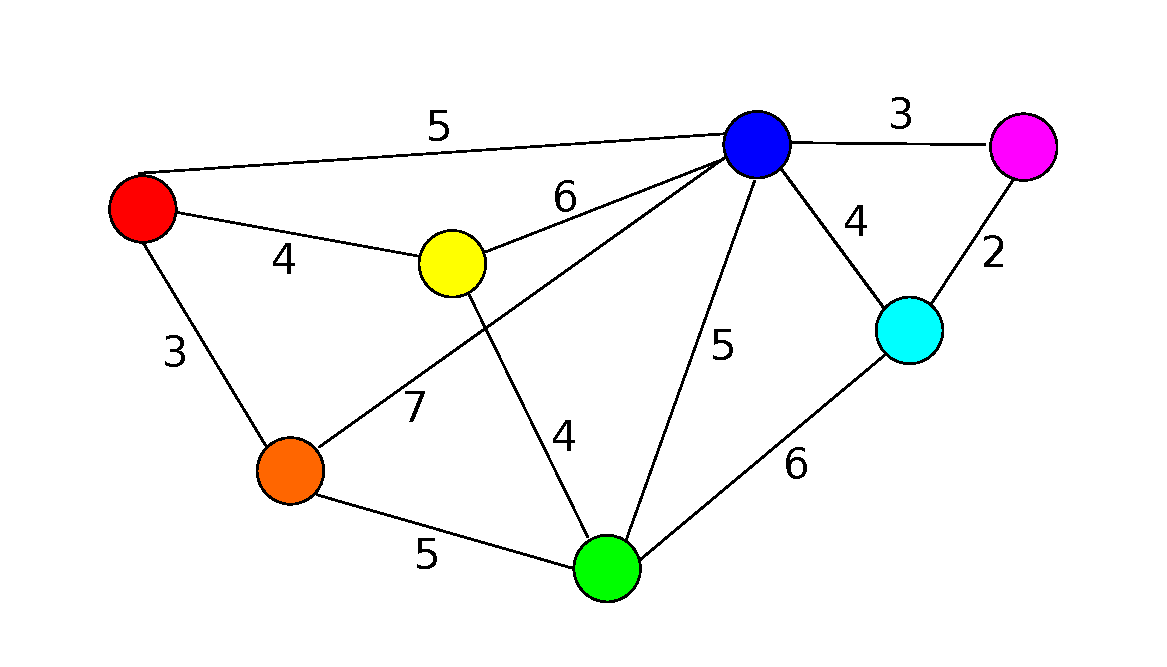
\includegraphics[width=3.0in]{weighted.pdf}}
	\textit{Yellow and Purple?}
        \begin{itemize}
	\item
		1. Yellow-Orange-Green-Indigo-Purple
	\item
		2. Yellow-Green-Blue-Indigo-Purple
	\item
		3. Yellow-Blue-Purple
	\item
		4. Yellow-Green-Indigo-Purple
	\end{itemize}
\end{frame}

\begin{frame}{Shortest Path Between...}
	\centerline{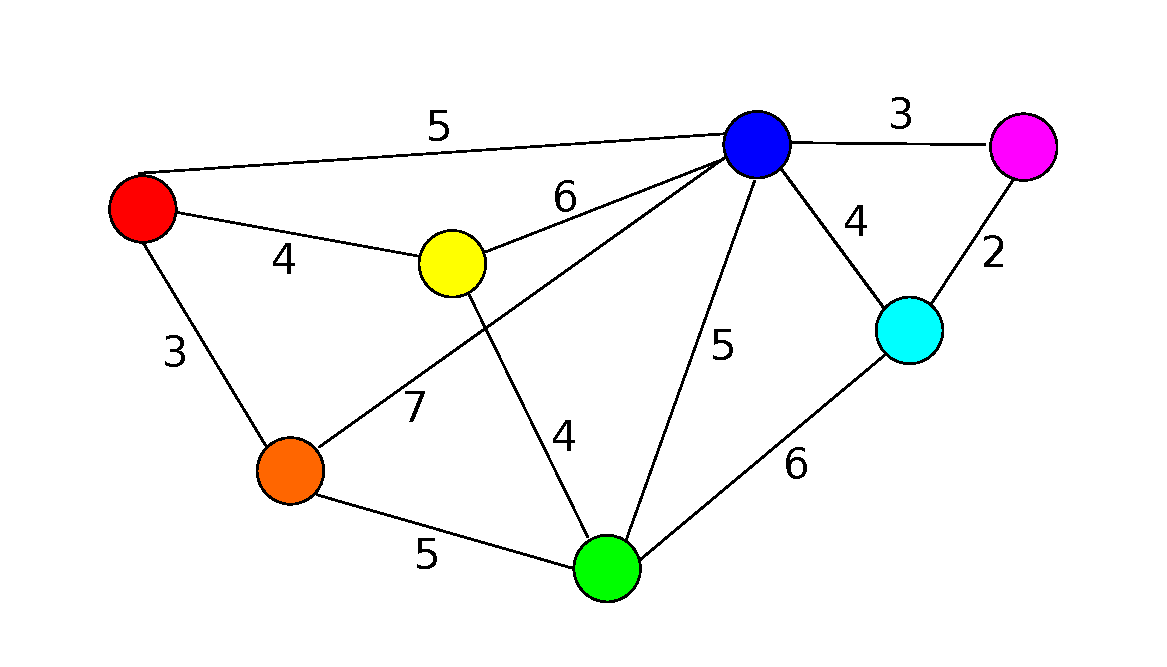
\includegraphics[width=3.0in]{weighted.pdf}}
	\textit{Yellow and Purple?}
        \begin{itemize}
	\item
		1. Yellow-Orange-Green-Indigo-Purple
	\item
		2. Yellow-Green-Blue-Indigo-Purple
	\item
		\alert{3. Yellow-Blue-Purple}
	\item
		4. Yellow-Green-Indigo-Purple
	\end{itemize}
\end{frame}

\begin{frame}{Shortest Path Between...}
	\centerline{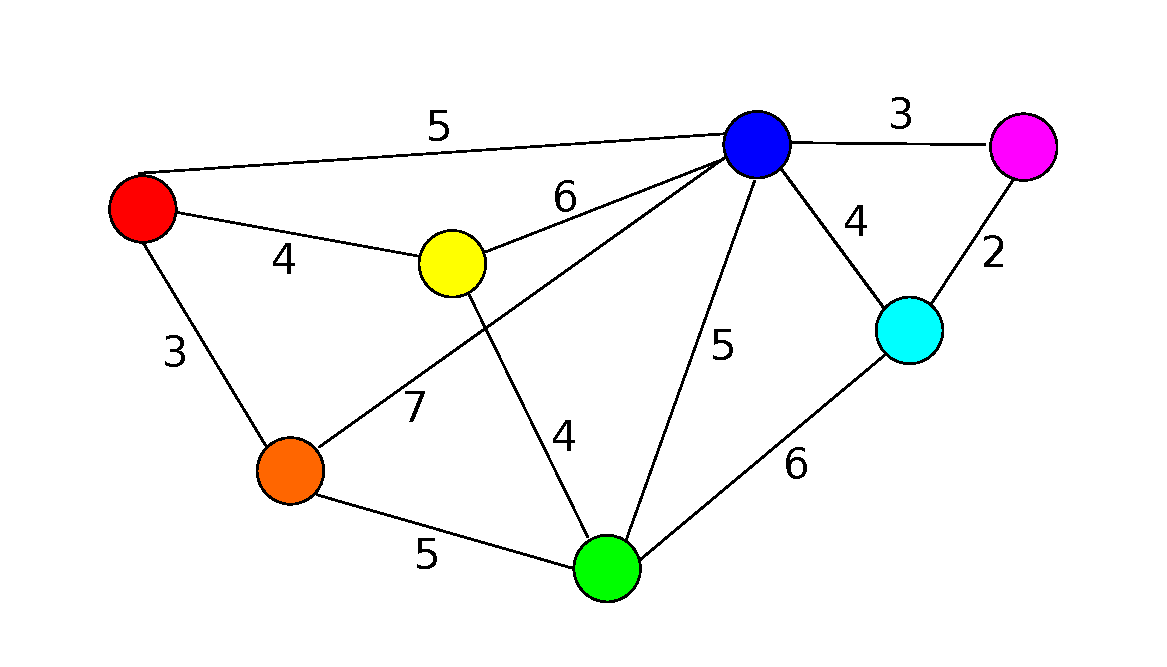
\includegraphics[width=3.0in]{weighted.pdf}}
	\textit{Indigo and Red?}
        \begin{itemize}
	\item
		1. Indigo-Blue-Orange-Red
	\item
		2. Indigo-Green-Blue-Yellow-Orange-Red
	\item
		3. Indigo-Purple-Blue-Red
	\item
		4. Indigo-Blue-Red
	\end{itemize}
\end{frame}

\begin{frame}{Shortest Path Between...}
	\centerline{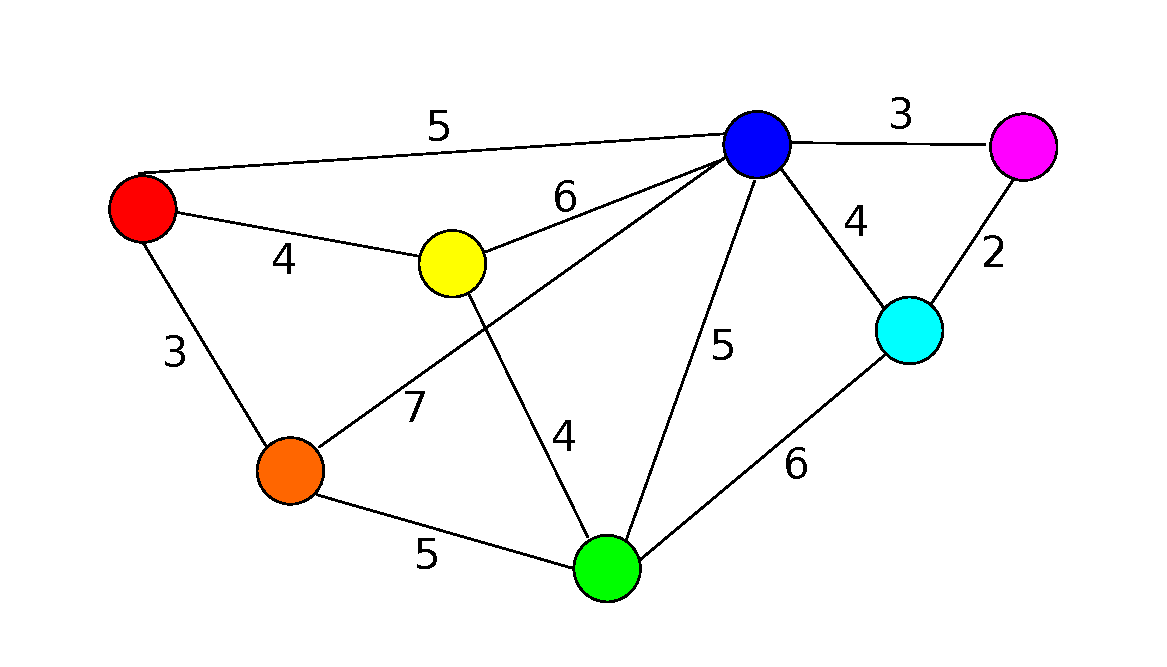
\includegraphics[width=3.0in]{weighted.pdf}}
	\textit{Indigo and Red?}
        \begin{itemize}
	\item
		1. Indigo-Blue-Orange-Red
	\item
		2. Indigo-Green-Blue-Yellow-Orange-Red
	\item
		3. Indigo-Purple-Blue-Red
	\item
		\alert{4. Indigo-Blue-Red}
	\end{itemize}
\end{frame}

\section{Dijkstra's Algorithm}
\subsection{Description}

\begin{frame}{History}
\begin{itemize}
\item
	Discovered by Dutch mathematician Edsger Dijkstra (1930-2002) in 1959.
\end{itemize}
\end{frame}

\subsection{Example}
\subsection{Python Code}
\subsection{Practice}

\section{The Traveling Salesman Problem}
\subsection{Description}
\begin{frame}{XKCD}
\centerline{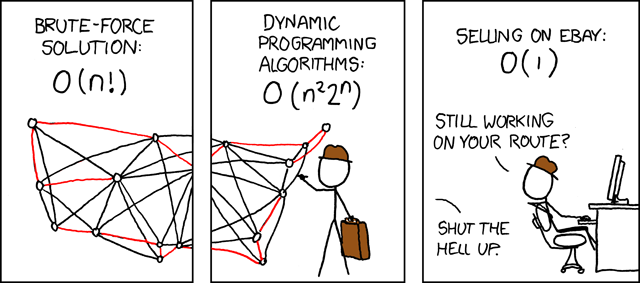
\includegraphics[width=3.5in]{travelling_salesman_problem.png}}
\end{frame}

\end{document}


